\documentclass[conference]{IEEEtran}
\IEEEoverridecommandlockouts
% The preceding line is only needed to identify funding in the first footnote. If that is unneeded, please comment it out.
\usepackage{cite}
\usepackage{amsmath,amssymb,amsfonts}
\usepackage{graphicx}
\usepackage{textcomp}
\usepackage{xcolor}
\def\BibTeX{{\rm B\kern-.05em{\sc i\kern-.025em b}\kern-.08em
    T\kern-.1667em\lower.7ex\hbox{E}\kern-.125emX}}
\title{
\vspace{1cm}
{
\includegraphics[width=0.15\textwidth]{ /storage/emulated/0/vignan/IMG-20241018-WA0001.jpg} \\ Assembly Assignment}}
\author{Bynaboyina Aiswarya \\ Roll No: FWC22295 \\ aiswaryabaiswarya61@gmail.com}
 \begin{document}
\maketitle
 \section{ABSTRACT}

This paper explains about the question asks for the 16-bit two's complement binary representation of the decimal number -28. The correct binary sequence must be identified. In two's complement, negative numbers are represented by inverting all bits of the absolute value of the number and adding 1 to the least significant bit.
The question can be implemented using assembly code in arduino uno and the correct binary sequence must be displayed in LCD [Liquid Crystal Display] - JHD 162A.

\section{COMPONENTS} 

The required components list is given in Table: I., pin diagram of LCD JHD 162A is shown in Fig.1.
\vspace{0.3cm}
 \begin{table} [htbp]
\centering
\begin{tabular}{| c | c | c |} \hline
Components & Value & Quantity \\\hline
LCD & JHD 162A & 1 \\ \hline
Arduino & UNO & 1 \\ \hline
Jumper Wires &  & 20 \\ \hline
Breadboard & & 1 \\ 
\hline
\end{tabular}
\vspace{0.3cm}
\caption{\label{tab:widgets}}
\end{table}

\section{PROCEDURE}
 \begin{enumerate}
\item Pin Configuration of LCD JHD162A.

\begin{figure}[h]                           
\centering                                 
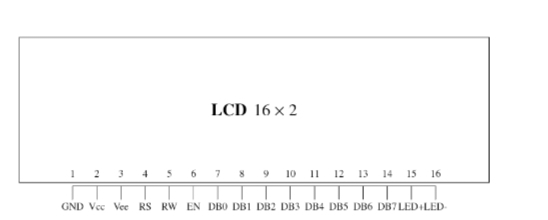
\includegraphics[width=0.5\textwidth]{/storage/emulated/0/vignan/IMG_20241021_151659.jpg  }                                           
\caption{\label{fig-1:Gates}}               
\end{figure}

\item Make connections of arduino uno to LCD 
JHD 162A as per below fig-2.

\begin{figure}[h]                           
\centering                                 
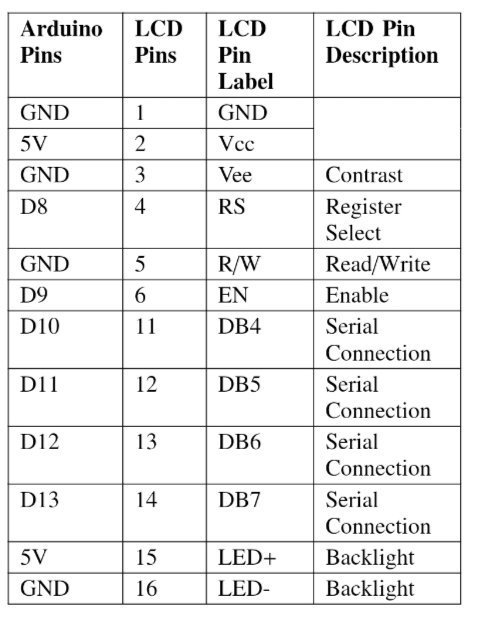
\includegraphics[width=0.4\textwidth]{ /storage/emulated/0/vignan/IMG_20241021_152652.jpg  }                                           
\caption{\label{fig-2:Gates}}               
\end{figure}


\item Execute the arduino code in nvim editor using avra filename.tex command.
\item After upload the code into hardware setup using arduino IDE platform.
 \end{enumerate}

\section{RESULTS}
 \begin{enumerate}
\item Download the codes given in the link below and execute them to see the output as shown in figure 3.
\item https://github.com/BynaboyinaAiswarya/Fwc-/blob/main/Assembly/main.asm
 \end{enumerate}


 \begin{figure}[h]                           
\centering                                 
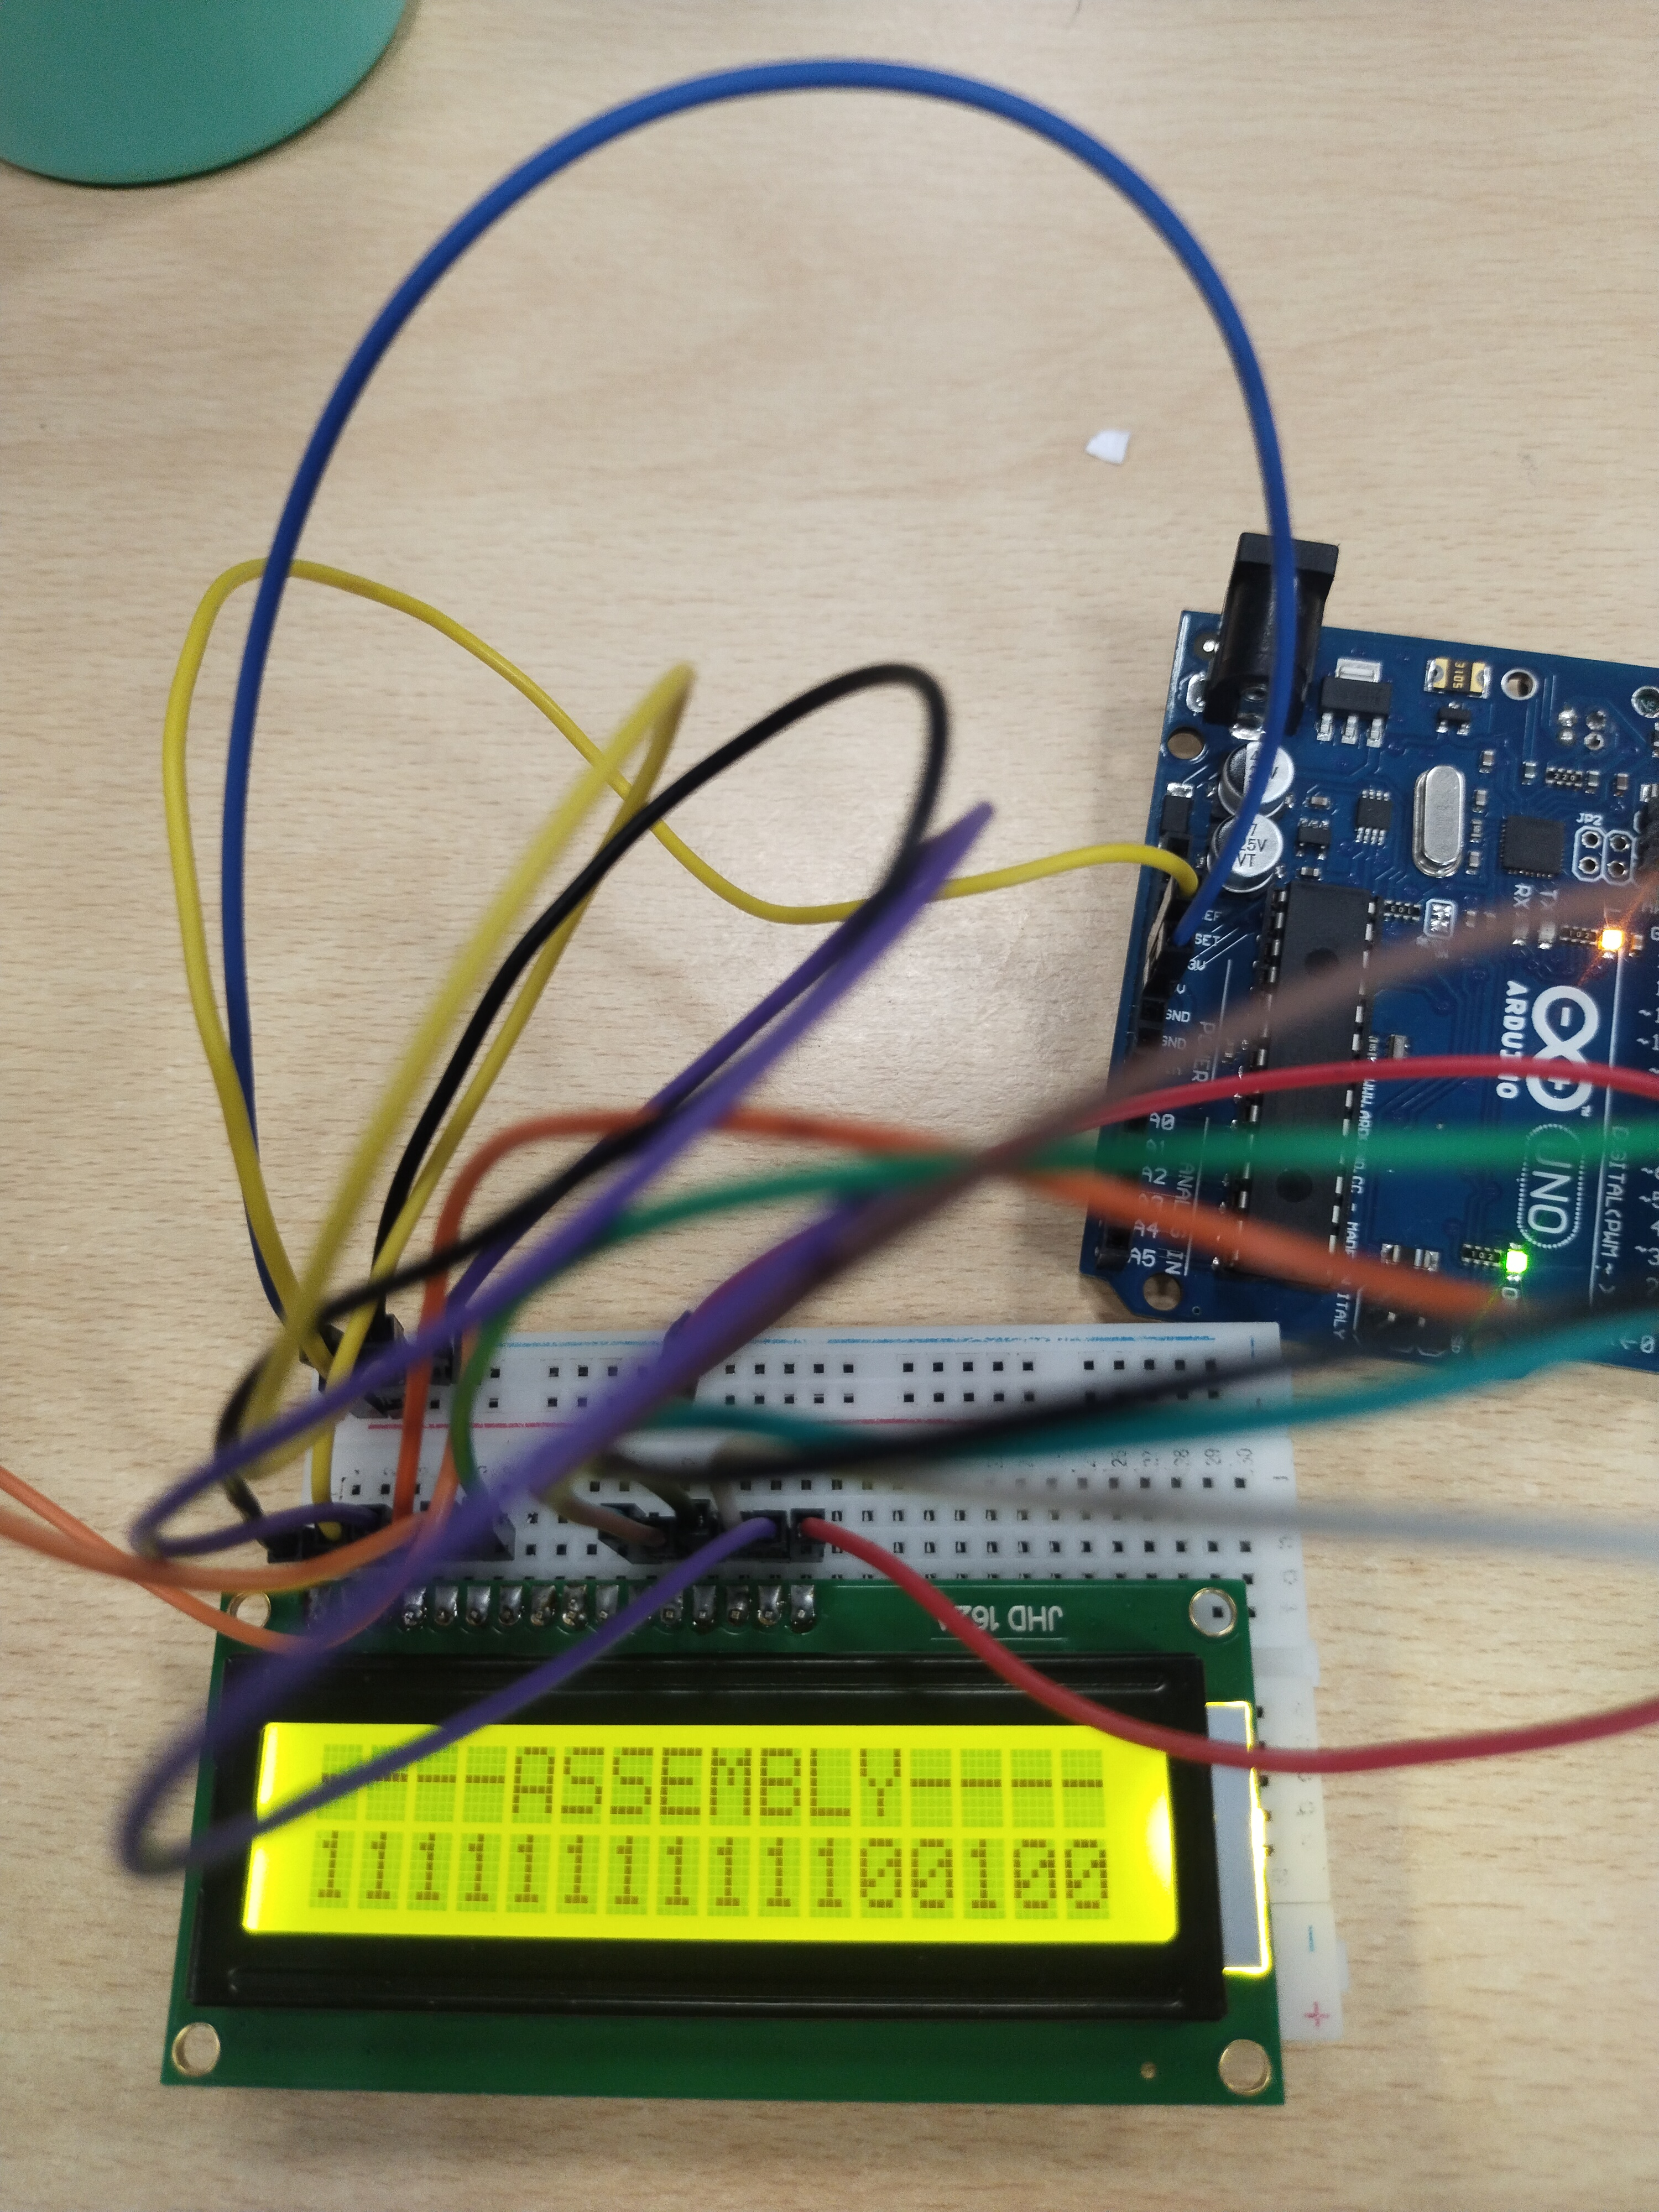
\includegraphics[width=0.4\textwidth]{ /storage/emulated/0/vignan/IMG_20240927_154157.jpg    }                                           
\caption{\label{fig-3:Gates}}               
\end{figure}
\section{CONCLUSION}
Hence implementation of assembly code in arduino uno and the correct binary sequence is displayed on LCD [Liquid Crystal Display] - JHD 162A is done .


\end{document}
